\input{../YKY-preamble-big.tex}
\setmainfont[BoldFont=Alibaba_Sans_Regular.otf,ItalicFont=Alibaba_Sans_Light_Italic.otf]{Alibaba_Sans_Light.otf}

% \usepackage[backend=biber]{biblatex}
% \bibliography{../AGI-book}

\usepackage[active,tightpage]{preview}		% for continuous page(s)
\renewcommand{\PreviewBorder}{0.5cm}
\renewcommand{\thempfootnote}{\arabic{mpfootnote}}

\usepackage[absolute,overlay]{textpos}		% for page number on upper left corner

\usepackage{color}
\usepackage{mathtools}
\usepackage[hyperfootnotes=false]{hyperref}

\usepackage{pict2e}		% pciture drawing polygon
% \usepackage[backend=biber,style=numeric]{biblatex}
% \bibliography{../AGI-book}
% \renewcommand*{\bibfont}{\footnotesize}

\usetikzlibrary{shapes}
\usepackage[export]{adjustbox}				% ??
\usepackage{verbatim} % for comments
% \usepackage{newtxtext,newtxmath}	% Times New Roman font

% \titleformat{\subsection}[hang]{\bfseries\large\color{blue}}{}{0pt}{} 
% \numberwithin{equation}{subsection}

\newcommand{\underdash}[1]{%
	\tikz[baseline=(toUnderline.base)]{
		\node[inner sep=1pt,outer sep=10pt] (toUnderline) {#1};
		\draw[dashed] ([yshift=-0pt]toUnderline.south west) -- ([yshift=-0pt]toUnderline.south east);
	}%
}%

\newcommand\reduline{\bgroup\markoverwith{\textcolor{red}{\rule[-0.5ex]{2pt}{0.4pt}}}\ULon}

%\DeclareSymbolFont{symbolsC}{U}{txsyc}{m}{n}
%\DeclareMathSymbol{\strictif}{\mathrel}{symbolsC}{74}
\DeclareSymbolFont{AMSb}{U}{msb}{m}{n}
\DeclareSymbolFontAlphabet{\mathbb}{AMSb}
% \setmathfont{Latin Modern Math}
\DeclareMathOperator*{\argmin}{arg\,min}

% For cover-page graphics
\def\Put(#1,#2)#3{\leavevmode\makebox(0,0){\put(#1,#2){#3}}}


% \usepackage[most]{tcolorbox}
\tcbset{on line, 
	boxsep=4pt, left=0pt,right=0pt,top=0pt,bottom=0pt,
	colframe=red,colback=pink,
	highlight math style={enhanced}
}
\newcommand{\atom}{\vcenter{\hbox{\tcbox{....}}}}

%\let\oldtextbf\textbf
%\renewcommand{\textbf}[1]{\textcolor{blue}{\oldtextbf{#1}}}

\newcommand{\logic}[1]{{\color{violet}{\textit{#1}}}}
\newcommand{\underconst}{\includegraphics[scale=0.5]{../2020/UnderConst.png}}
\newcommand{\KBsymbol}{\vcenter{\hbox{\includegraphics[scale=1]{../KB-symbol.png}}}}
\newcommand{\token}{\vcenter{\hbox{\includegraphics[scale=1]{token.png}}}}
\newcommand{\proposition}{\vcenter{\hbox{\includegraphics[scale=0.8]{proposition.png}}}}

\newcommand{\circled}[1]{{\textcircled{\sffamily \scriptsize{#1}}}}

\newcommand{\egg}[1]{\footnotesize #1 \normalsize}

\setcounter{secnumdepth}{0}		% no section 

\begin{document}

\begin{preview}

\title{\vspace{-1.5cm} \bfseries\color{blue}{\LARGE Global AGI Project}}

% \author{YKY} % Your name
\date{\vspace{-2cm}} % Date, can be changed to a custom date

\setcounter{section}{-1}
\newcounter{mypage}
\setcounter{mypage}{1}

% (1) Circled page number on upper left corner
% \begin{textblock*}{5cm}(2.1cm,2.3cm) % {block width} (coords) 
% {\color{red}{\large \textcircled{\small 1}}}
% \end{textblock*}

%\begin{minipage}{\textwidth}
%	\setlength{\parskip}{0.4\baselineskip}
%
%	\begin{picture}(600,220)
%	\put(0,65){\includegraphics[scale=1]{../2021/Genifer-square-logo.png}}
%	\definecolor{graygray}{rgb}{.867,0.867,0.867}
%	{\color{graygray}\polygon*(-55,-80)(-55,-5)(400,110)(400,-80)}
%	\Put(215,-105){\includegraphics[scale=0.08]{../2021/robot1.jpg}}
%	\end{picture}
%\end{minipage}
%\end{preview}
%\begin{preview}

\begin{minipage}{\textwidth}
\setlength{\parskip}{0.4\baselineskip}
\section{新新皮质 \quad \quad \small{Neo-neocortex}}

强人工智能 将会在数月~一两年内出现。\\
\egg{Strong AI may arrive in 1-2 years or even within months.}

届时,所有工作都会被 自动化,没有例外。\\
\egg{By then, all known jobs will become automated, with no exceptions.}

人类如要避免淘汰,必需跟 AI 融合,\\
此即我所提出之 neo-neocortex 概念: \\
\egg{If humans were to avoid being out-competed, we must integrate with AIs.  This is what I called the ``neo-neocortex'':}
\begin{equation}
\nonumber
\vcenter{\hbox{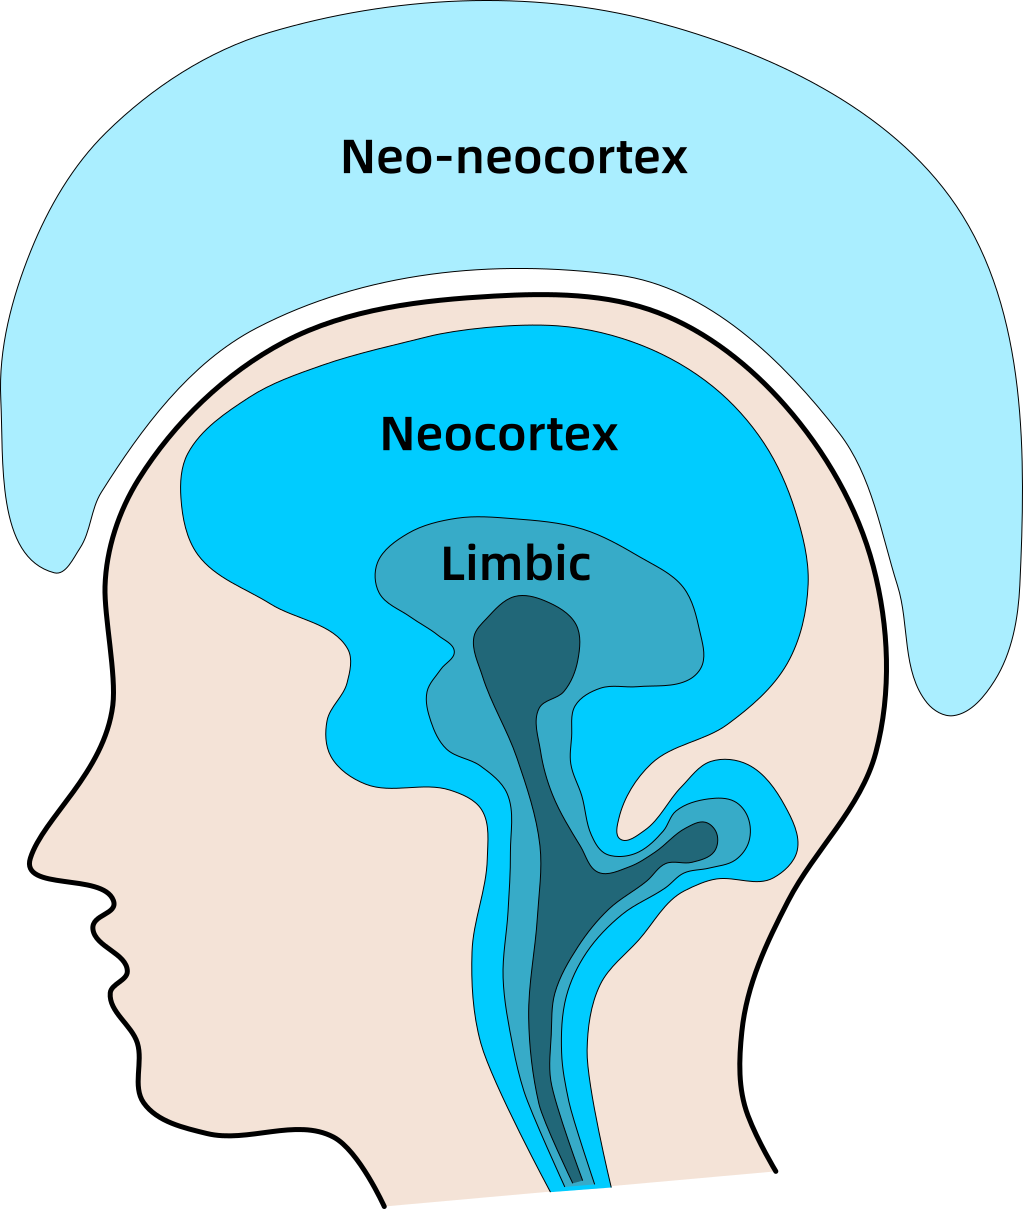
\includegraphics[scale=0.6]{neo-neocortex.png}}}
\end{equation}
但它不一定直接连接着大脑,而是抽象意义上的。\\
\egg{Though it may not mean directly or physically connecting with the brain, but in an abstract sense.}
\end{minipage}
\end{preview}

\begin{preview}
\begin{minipage}{\textwidth}
\setlength{\parskip}{0.4\baselineskip}

\section{香港在全球化环境下的角色 \\ \hspace*{5cm} \small{The role of Hong Kong in the global AI milieu}}

目前,高科技是被 美国霸权 垄断的。\\
\egg{In the present world, American hegemony has a monopoly over high-technologies.}

AGI 人材 主要流向 英-美 为主的企业:
\begin{equation}
\nonumber
\vcenter{\hbox{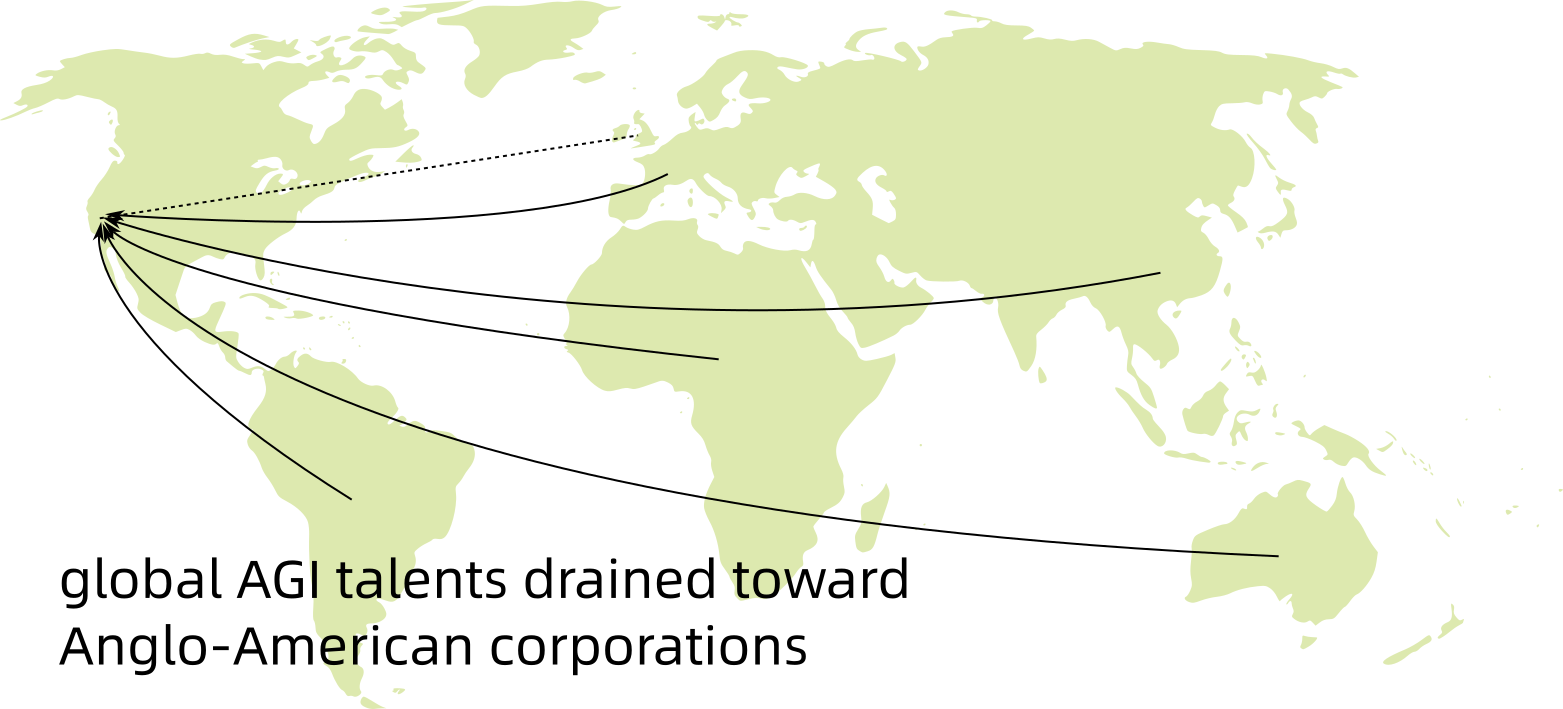
\includegraphics[scale=0.7]{global-AGI-talent-drain-En.png}}}
\end{equation}

尽管人们觉得美国是个 进步开明的国家,但近日 以色列问题 清楚地 暴露了 美国其实有顽固的种族歧视的一面。 美国的 \textbf{理想} 跟 美国的 \textbf{现实},之间存在了一段不少的距离。\\
\egg{Although people generally think of America as an advanced and progressive nation, the recent Israeli-Palestinian conflict exposed a darker, racist side. There exists a considerable gap between America's \textbf{ideal} and America's \textbf{reality}.}

地球上很多国家其实也缺乏打破美国霸权的实力,包括中国、俄罗斯、日本、欧洲 等。 但 AGI 是一种极为重要的技术,它的重要性甚至超过 工业革命、农业的出现、甚至火的使用。 这个世界很需要一个独立于美国的 AGI 项目,特别是着重 种族平等 的。\\
\egg{Many countries of the world lack the power to compete with American hegemony, that includes China, Russia, Japan, Europe, etc.  But AGI is an extremely important technology, comparable to the industrial revolution, emergence of agriculture, or even the use of fire. Our world needs an independent AGI project with special emphasis on racial equality.}

而中国并不具备发展 AGI 的土壤,因为它的社会结构仍然是高度封闭的、人民的思想并不尊重科学。 正如 Conway's Law 所说:一个组织生产的产品,会不自觉地模仿它本身内部沟通的方式。那么中国或许做不出 AGI、或许会做出压抑人民的 AGI 系统。\\
\egg{China is not a suitable soil for developing AGI, because Chinese society is still highly isolationist, its people generally do not highly regard scientific ideas. As \textbf{Conway's Law} says: an organization tends to produce products that mimic its internal communication structure.  China may fail to produce AGI, or likely to create an oppressive one.}

\end{minipage}
\end{preview}

\begin{preview}
	\begin{minipage}{\textwidth}
		\setlength{\parskip}{0.4\baselineskip}
		
		\section{AGI 理论 \hspace*{4cm} \small{Some AGI theory}}

LLM 就像 盲聋女作家 Helen Keller,她唯一感知外界的渠道 就是「预测下一个词」。\\
\egg{LLM is like the blind-deaf writer Helen Keller, her only sensory window to the external world is ``to predict the next word.''}

预测世界 其实等同于 建立 \textbf{世界模型}。强化学习的目标 是最大化以下的 Bellman 条件:
\begin{equation}
\nonumber
\max_{\pi} \; \underset{\substack{a_t \;\sim\; \pi(\cdot | s_t) \\ s_{t+1} \;\sim\; p(\cdot | s_t, a_t) }} {\mathbb{E}} \left[ \sum_{t} \gamma^t R(s_t, a_t) \right]
\end{equation}
换句话说,RL 就是学习 $p$ 和 $\pi$. 其中 $\pi$ 是策略,$p$ 就是 世界模型。\\
\egg{To predict the world is to construct \textbf{world models}. The objective of reinforcement learning is the Bellman condition, where we need to learn $\pi$, the policy, and $p$, which is the world model.}

建立 世界模型 的算法,跟现在流行的 generative models 原理是一样的。例如 autoencoder 或 diffusion model 都是这家族成员。
\begin{equation}
\nonumber
\vcenter{\hbox{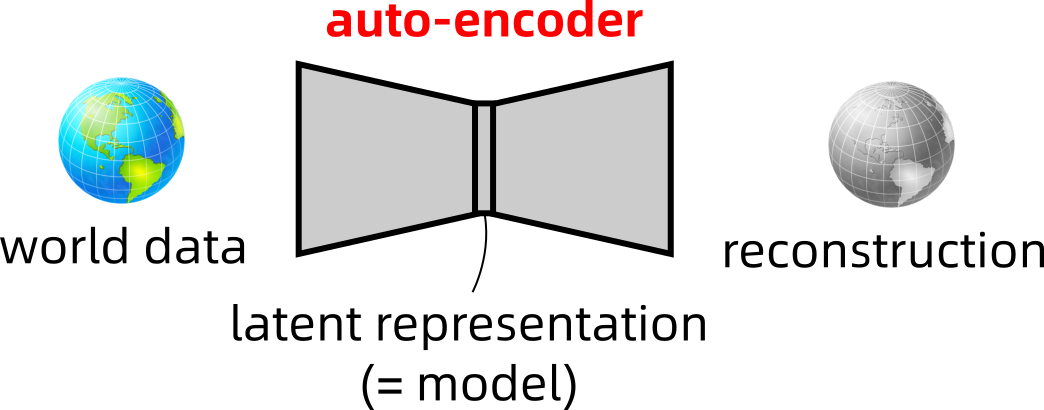
\includegraphics[scale=0.7]{auto-encoder.png}}}
\end{equation}
\egg{The principles behind building world models are the same as those for the currently popular \textbf{generative models}, with special cases such as auto-encoders and diffusion models.}

有趣的是,其实人脑就是一个这样的「自编码器」: 感觉资料 经过层层的、越来越抽象的处理,然后 这些抽象的特征 再 \textbf{反向传播} 回到 感知区域,这结构相当于一个中间对褶起来的 自编码器。
\begin{equation}
\nonumber
\vcenter{\hbox{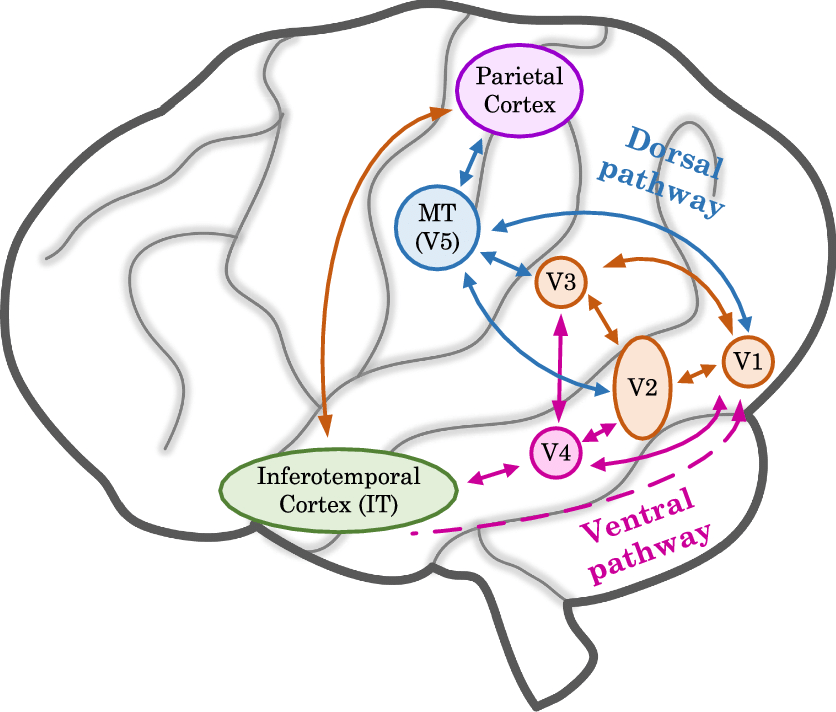
\includegraphics[scale=1]{visual-cortex.png}}}
\end{equation}
\egg{Interestingly, the human brain is just such an auto-encoder: sensory information is processed by a hierarchy of increasingly abstract representations, which abstract features are \textbf{back-projected} to primary sensory areas, forming an auto-encoder folded in the middle.}

LLM 的成功证明 我们已经进入了 AGI 的「射程范围」之内。 AGI 在短期内是必然会出现的。 这不是我在吹嘘,大家用脑想想就会明白。\\
\egg{The success of LLMs proves that we have entered the ``ballpark'' of AGI, which is certain to arrive within a short time window.  This is not just my hyperbole, you can decide by your own thinking.}

目前重要的不是细节的争拗,而是将人材汇聚到一个项目里。
\egg{What we need now is not to argue about details, but to create a project to consolidate talented people.}

	\end{minipage}
\end{preview}

\begin{preview}
	\begin{minipage}{\textwidth}
		\setlength{\parskip}{0.4\baselineskip}
		
		\section{AGI:最后一步 \hspace*{4cm} \small{AGI: the last step}}

现时 LLM 首要的问题是「幻觉」的产生,解决这问题的原则性方法是将 LLM 放在 \textbf{强化学习} 的框架里,RL 的「回路」迫使其内部知识达致逻辑上的「\textbf{融洽性}」,从而消除知识里的矛盾及辨识谬误。这是通往 AGI 的最后一步。\\
\egg{The current ``pain point'' of LLMs are hallucinations, and the principled way to resolve this is to put LLMs inside the reinforcement learning framework, where the ``loop'' will force its internal knowledge to attain \textbf{logic coherence}, thus eliminating contradictions and able to discern falsehood.  This is the final step towards AGI.}

我自大约 20年前开始,从研究 经典 逻辑 AI 走来,很熟悉这背后的理论。\\
\egg{I began researching AGI nearly 20 years ago, starting from the classical logic-based AI tradition, so I am very familiar with this theoretical background. }

现时的障碍是如何将 LLM 嵌入 RL 架构里。 在这方面我做了不少实验\footnote{http://github.com/Cybernetic1/reinforcement-learning-experiments} 和思考。 我一直提出的理论是利用 \textbf{交换对称性} 切割搜寻空间,从而加速学习(众所周知,Transformer或更一般的图神经网络 具有这种 交换对称性)。 但到了今天下午我才意识到,我的实验结果其实证明了这个想法是不成立的。 Transformer 并不是更快,但它更 \textbf{节省记忆} 而已。 
\begin{equation}
\vcenter{\hbox{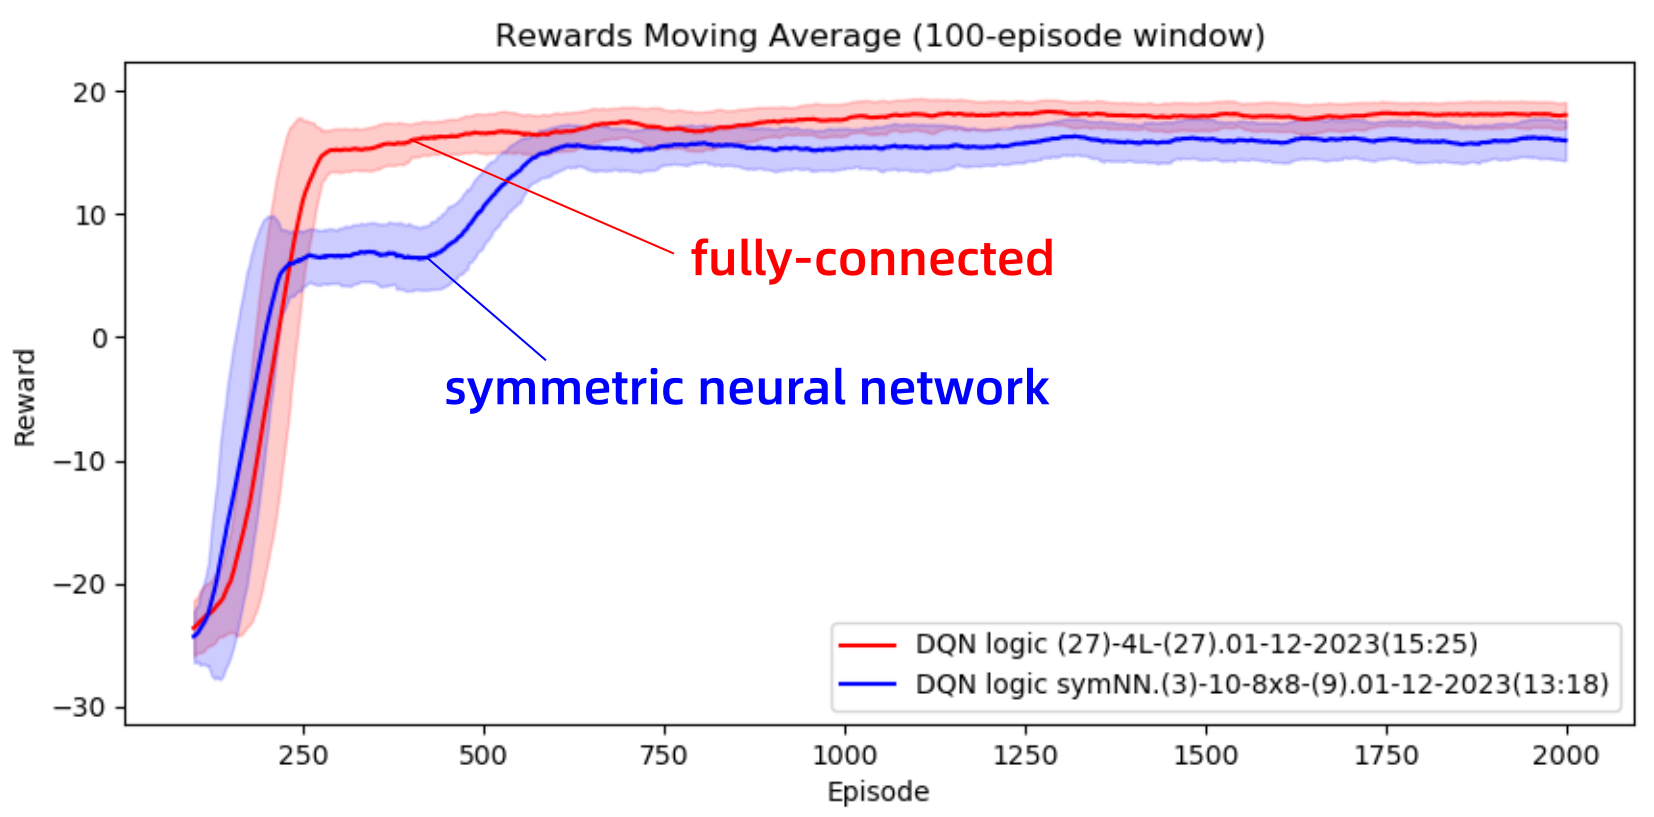
\includegraphics[scale=0.7]{symmetric-vs-full2.png}}}
\end{equation}
\egg{The current obstacle is how to fit LLM into RL, for which I have done a lot of thinking and experimentations$^1$. I have been pursuing the idea of using \textbf{permutation symmetries} to reduce the size of hypothesis space, thus accelerating learning.  As is well known, the Transformer possesses this type of invariance.  But this afternoon I realized that this idea is refuted by my own experiments.  The Transformer is not really faster; it is just more \textbf{memory-efficient}.}

另一个问题是「思维空间」是非常大、或近乎无限的离散空间,它近似于连续空间。 很多 强化学习 算法不能处理 连续动作。我提出 直接输出动作空间上的概率分布,并将「思维」分拆成符号的概率分布(沿用 Transformer 的思路)。\\
\egg{Another problem is that the ``mental space'' is an enormous, almost infinite discrete space, which is close to continuous, and many RL algorithms cannot handle continuous actions. I propose to directly output the action probability distribution, and decompose each ``thought'' into constituent symbols (along the Transformers' line of approach).}

我的理论暂时只能用 井子棋 试验,如用 LLM 则需要很多 GPU,在这方面 HKAI Lab 能给我们关键的帮助。\\
\egg{Right now we can only use TicTacToe experiments to verify our theory. LLM would require more GPUs, which is an area that HKAI Lab can help us crucially.}

	\end{minipage}
\end{preview}

\begin{preview}
	\begin{minipage}{\textwidth}
		\setlength{\parskip}{0.4\baselineskip}
		
% 		\section{?? \hspace*{4cm} \small{???}}

\subsection{Business model}

\begin{itemize}
	\item Our business is to run a GPT-like server to serve the global public, as an alternative to eg. OpenAI.
	
	\item Subscription model.
	
	\item The costs of running the server depends on volume of texts processed.
	
	\item We try to do R\&D on the models and algorithms while running the server commercially.  The superiority of our algorithms, if our theory is correct, differentiates us from other competitors.  This seems to be the only way to develop an ability to research on AGI.  Without this ability, we would always be at the mercy of other companies' innovations.
	
	\item We may not physically build the server; rather we rent computer servers to run our algorithms and sub-let our services to the public.
	
	\item We could utilize distributive computing and crypto-currencies.  We developed a web platform for distributive collaboration (``Snow-Crossing'', applied for HKAI Lab before) as a DAO (decentralized autonomous organization)

\end{itemize}

长久以来,我得不到任何资助,因为香港人觉得我做的事是不可企及的,他们觉得我谈 AGI 就像在讲外星人语言。他们喜欢培养一些 刻意避开外国竞争的商务,结果长远来看,他们仍然没有进步。\\
\egg{Hong Kong people tend to think my ambitions are unfeasible, as if I'm talking in an alien language. They tend to invest on businesses that carefully avoid competition with the West, but they end up being unable to grow technologically. }

技术不是喜欢抄袭就能抄袭到的,所以我们要培养自主研发的能力,尤其现在美国已意识到 AI 技术是商业秘密。\\
\egg{Technology is not something that we can plagiarize at will, it requires time to build up knowledge and expertise in teams.  The need to develop our own R\&D is more important now that Americans start to recognize AI as trade secrets.}

香港投放在高科技的资源很短缺,而我完全得不到任何资助,这是不合理的。 \\
\egg{The resources HK invests in high tech are very scarce to begin, but that I receive 0\% allocation of it is unreasonable.}

There are more details that we can discuss in an interview.  Hope to see you around :)

% 一个国家 进步的程度,在于其文化接近「真实」的距离。 落后国家人民的思想不科学,所以办起事来效率很低。 香港人觉得祖国落后、屏蔽外界资讯 是很可耻的事,然而香港人自己是不是也固步自封?

%中国学术界有个奇怪现象,就是大家很有默契地假装外国竞争不存在,然后努力在做自己的「研究」。 在这种情况下 做假 成为了常态,是不能根治的。 

%我成长于 1970-80 年代的香港,那时候香港人见到外国人会害怕到脚软。 现在很多香港人听到我提起这件事会哈哈大笑,事实是,香港仍未脱离这种心态,仍然在逃避跟外国竞争、这样发展下去跟内地仍是没有分别。

%究其原因,就是进步的人被其他人妒忌而被「拖下去」。 这种心态是因为很多人觉得所有人都应该一样落后,否则是「不公平」。 

	\end{minipage}
\end{preview}

\begin{preview}
	\begin{minipage}{\textwidth}
		\setlength{\parskip}{0.4\baselineskip}
		
		\section{AGI 理论 \hspace*{4cm} \small{Some AGI theory}}
		
	\end{minipage}
\end{preview}


\begin{preview}
\begin{minipage}{\textwidth}
\setlength{\parskip}{0.4\baselineskip}

\maketitle

\section{About Myself}

\begin{itemize}

	\item Hello. This is me, some years ago, in HKU library: \\
	\begin{equation}
	\nonumber
	\vcenter{\hbox{\includegraphics[scale=0.5]{/home/yky/self/AI4U.jpg}}}
	\end{equation}

	\item You might have noticed I have been applying to every cohort of this program.
	
	\item But this is the first time I pitch on the business idea that is my true passion, which is AGI.
	
	\item In the past attempts, I have tried to disguise AGI under other business ideas because somehow I wanted to approach AGI from an oblique angle, to perhaps squeeze into your incubation program.  And also because I don't want to pitch an idea that sounded like blue-sky research or that I'm out of touch with reality.  But this is no longer necessary.  The time is now ripe for AGI.
	
	\item I have started independent research on AGI in earnest, since 2004.  During the past ~20 years there was never a day I did not work on AGI.
	
	\item Hong Kong is a technologically very backwards place (not in the sense that people do not own slick cell phones, but we are not part of the developers of these technologies).  Perhaps this is a too-harsh criticism, since basically the rest of the world can be said the same, except for USA, which dominates most high tech industries.  For a long time I could not find any partners or sponsors to work on AGI.  Not only that I received no help, but often sarcasm and bitterness from my fellow citizens as well.
	
	\item Maybe the number of people interested in AGI in HK is not exactly zero, but if this number is too small, then practically I really cannot find anyone with a similar interest.  I have cried over this every day for many years.  Perhaps, HKAI Lab has a bit of a responsibility to provide an opportunity to draw such talents together?
	
\end{itemize}
\end{minipage}
\end{preview}

\begin{preview}
\begin{minipage}{\textwidth}
	\setlength{\parskip}{0.4\baselineskip}

\section{AGI}

\begin{itemize}
	
	\item Assuming the reader is not an expert in AGI, I might explain it this way:  I think the development of AGI has reached a stage now where ``bottlenecks'' no longer exist.  In the past there were so-called ``bottlenecks'' in the sense that theoretical obstacles existed for which we cannot foretell their solutions.  But such obstacles no longer exist and we're at a stage of just \textbf{engineering} AGI systems, using tools and techniques that has been demonstrated to work and are reasonably well-understood.

	\item At this point it is important to design a \textbf{cognitive architecture} where researchers can clearly understand the internal workings of an AGI, for example, what is ``working memory'' and where is it located in the architecture, etc.
	
	\item I have independently proposed the ideas that \textbf{LLMs} (large language models) are ``world models'' in model-based reinforcement learning, and that Transformers can be seen as performing the function of \textbf{logic} rule-bases.  These are the core ingredients of an AGI.  Moreover, I proposed a way to treat ``thinking'' as ``actions'' in mental space, unifying thinking and acting under reinforcement learning.  My theories have been extensively published on 知乎.com (in addition to the AGI International Conference) which attracted a moderate following.  For example:  \href{https://zhuanlan.zhihu.com/p/615327294}{AGI 架构综述}
	
	\item Our basic architecture is as follows: (the long-term memory part has been demonstrated to work in Google's recent paper ``\textit{Memorizing Transformers}'')
	\begin{equation}
	\nonumber
	\hspace*{-1.6cm}
	\vcenter{\hbox{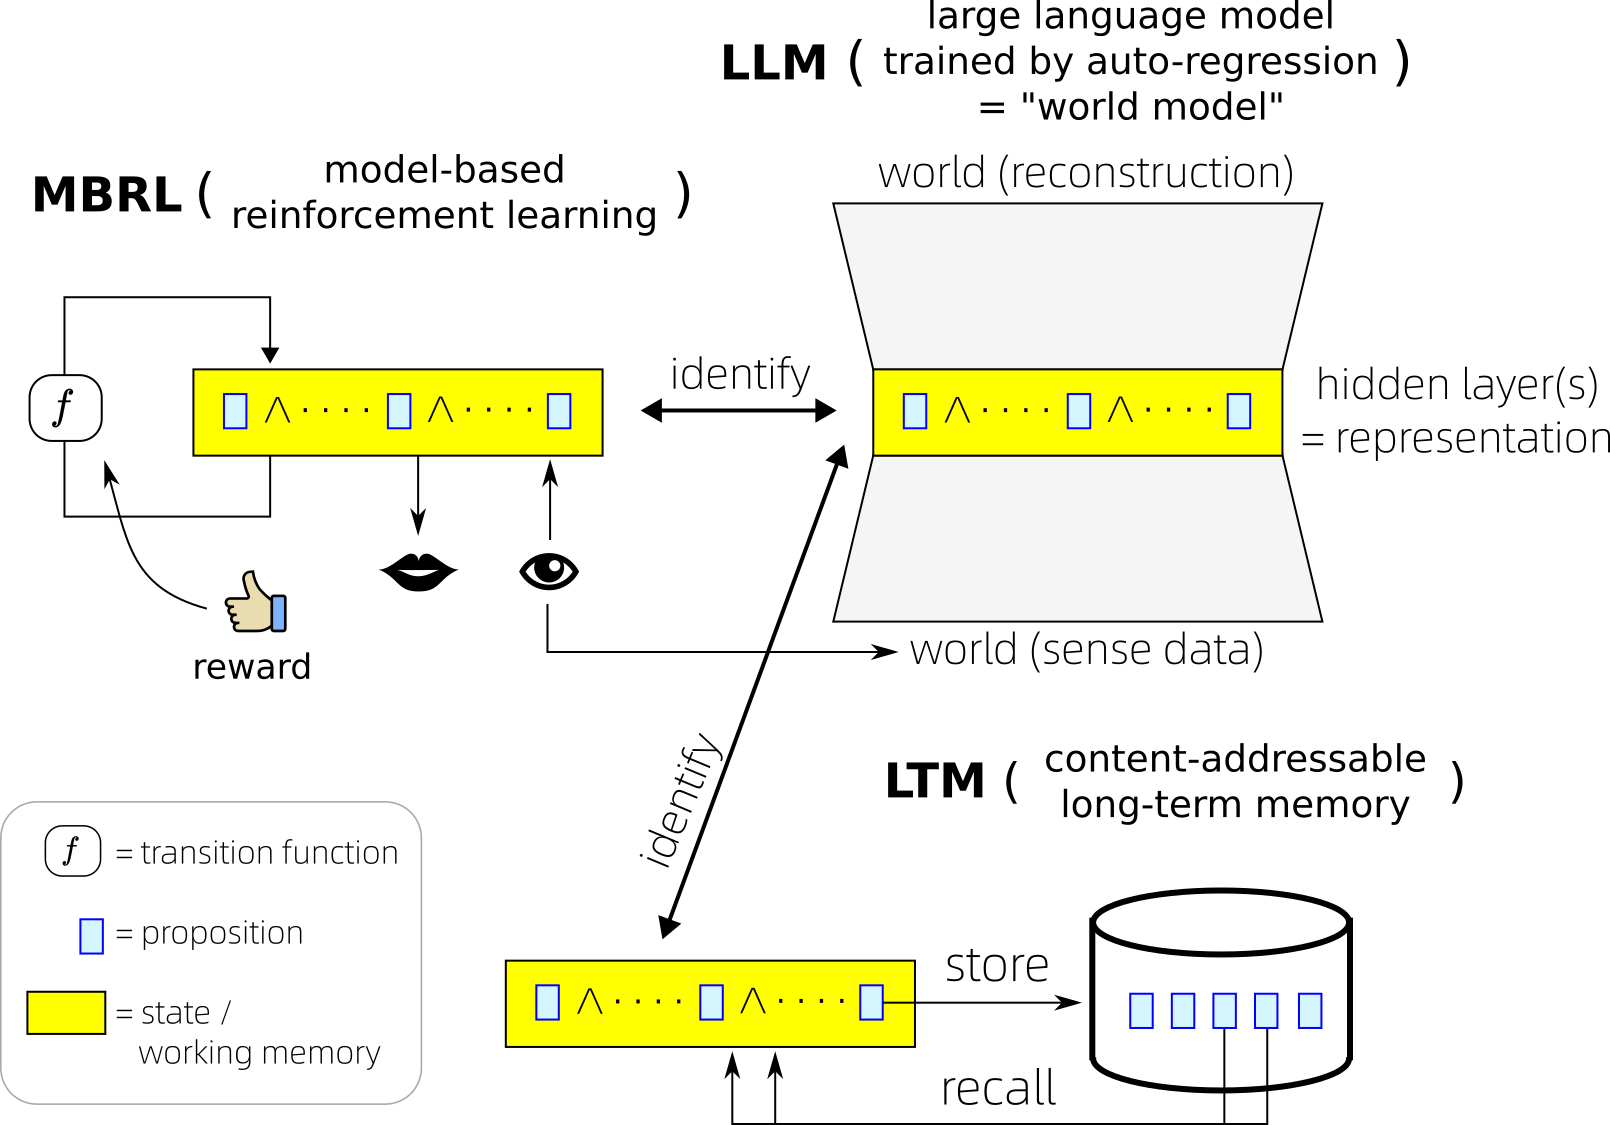
\includegraphics[scale=0.9]{AGI-architecture-LLM-MBRL-LTM.png}}}
	\end{equation}

%	\item This is the first prototype architecture we plan to build:
%	\begin{equation}
%	\nonumber
%	\hspace*{-1.6cm}
%	\vcenter{\hbox{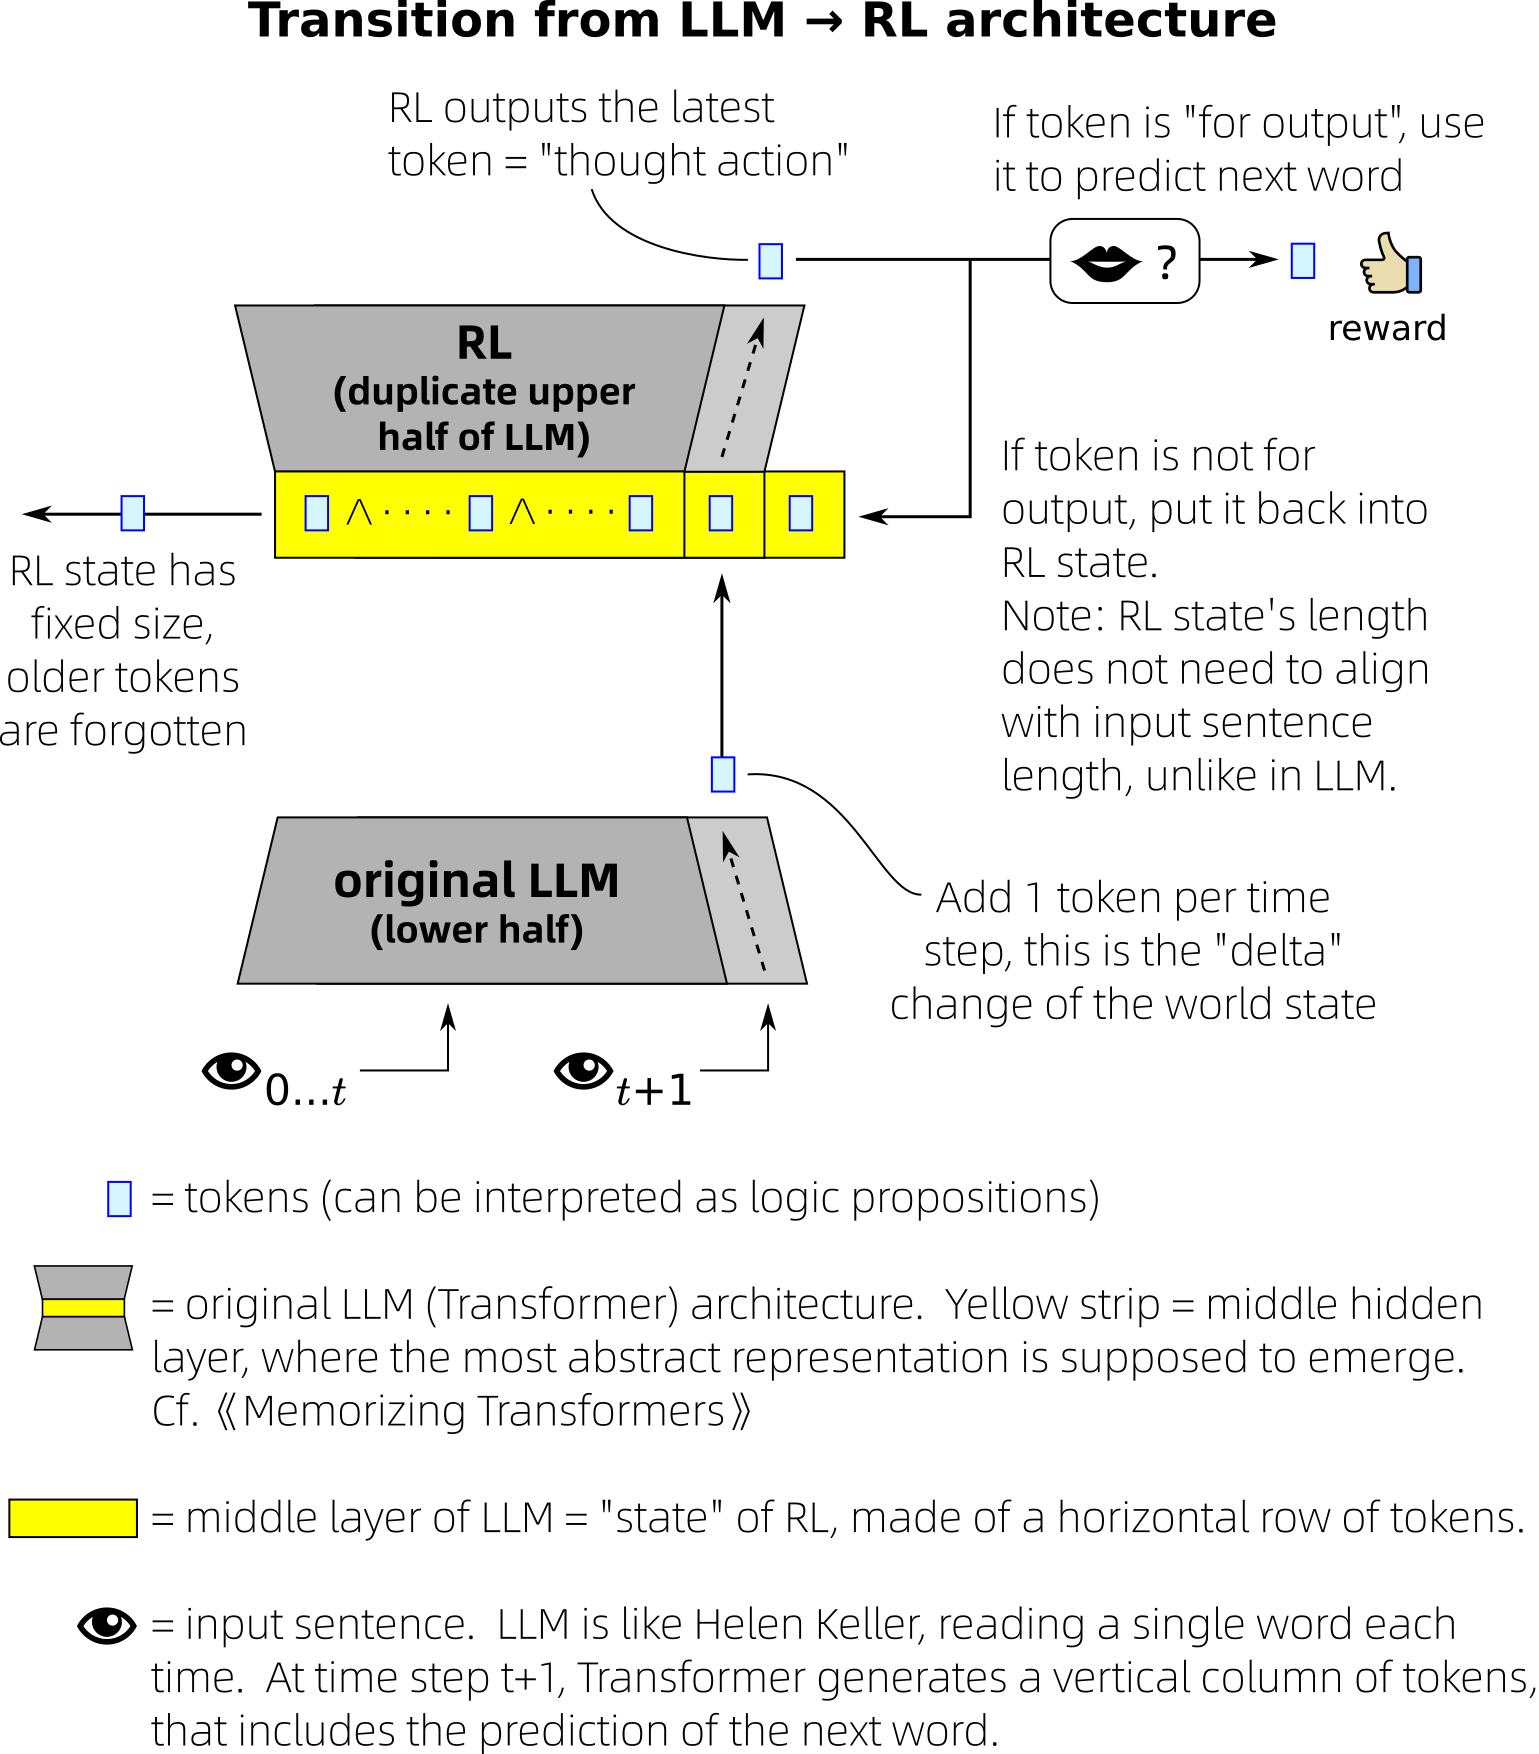
\includegraphics[scale=1]{LLM-to-RL-transition-architecture.png}}}
%	\end{equation}
		
\end{itemize}

\end{minipage}
\end{preview}

\begin{preview}
\begin{minipage}{\textwidth}
\setlength{\parskip}{0.4\baselineskip}
		
\section{Why Global?}

\begin{itemize}
	\item There is a widely recognized danger of AGI getting too strong and causing human catastrophes:
	\begin{equation}
	\nonumber
	\vcenter{\hbox{\includegraphics[scale=1]{../humanities/AGI-safety-EN.png}}}
	\end{equation}

	\item The only sensible solution for this problem seems to be to allow a \textbf{diversity} of AGIs trained with different value systems by humans.

	\item There is no operable definition that can distinguish between human \textbf{emotions} and machine emotions -- they are just reward functions in reinforcement learning -- implying that as AGI attains higher cognitive powers (including self-consciousness) they could become indistinguishable from human beings.  It is important to allow humans to represent their culture and values globally and adequately.

	\item Currently the USA (or Anglo-American companies) dominates the global technological landscape, especially in the field of AI.  This may pose a threat to diversity if there is a systematic bias towards Anglo-American values.  Another weakness may come from the homogeneity of AGI architectures designed by similar companies.  It would be beneficial for humanity as a whole if there is a globally collaborative AGI project.

	\item \textbf{Hong Kong}'s special position at the intersection of East and West makes it an ideal place to launch this global AGI project.  But, many Hong Kongers suffer from a psychological inferiority complex left over from colonialism, that makes them extremely averse to standing up against racism or challenging Anglo-American dominance, even though what I propose to do is positively regarded by many Westerners as the trend of the future.

\end{itemize}

\end{minipage}
\end{preview}


\begin{preview}
\begin{minipage}{\textwidth}
	\setlength{\parskip}{0.4\baselineskip}

\section{Our Team / Current State of Our Project}

\begin{itemize}
	\item 160 members in WeChat group, mostly students and researchers of AGI, mainly from mainland China

	\item An international team is also in the process of forming, on Telegram and Discord. (I used to have an international AGI research team circa 2000's)
	
	\item 1-2 angel investors (from mainland China)

	\item AGI prototype planned to complete training in mid-May this year (2023).  The main point of the demo is integrating reinforcement learning with LLM according to our AGI theory.

	\item We are forming partnerships (indeed, an ecosystem) in business applications of AGI, such as simple businesses utilizing GPT-like services, AIGC, and Web3 technologies (our own AGI project is operated as a DAO -- distributive autonomous organization).

\end{itemize}

\end{minipage}
\end{preview}
\end{document}
